\subsection{A nova solução}

  Em função das limitações de tamanho e tempo, observou-se uma oportunidade para utilização de abordagem baseada em metodologias ágeis. No entanto, não é objetivo discorrer sobre o andamento de um projeto de software em sua completude mas, focar em algumas técnicas de desenvolvimento utilizadas. De tal forma, contamos com uma certa indulgência do leitor no que se refere a omissões descritivas dos caminhos gerenciais tomados.

  Usando \emph{histórias de usuário} como método de requisitos observamos a existência de muitas delas, de tal forma que se faz necessário organizar as mesmas dentro de um fluxo de capacidade mínimo \footnote{\citeonline{Patton2014} apresentam uma técnica, \emph{Mapeamento de Histórias de Usuário}, bastante útil para identificar fluxos e definir sua importância, em particular para o contexto em que não existe um proprietário de projeto - PO - capaz de priorizar as histórias que mais lhe agregam valor.} para completar as intenções firmadas no escopo. Daí se chega à \textbf{Figura \ref{fig:mapeamento-historias-usuario}}, onde se observa que 7 histórias são essenciais: \emph{criar conta; entrar; sair; chamar partida; atender chamado para partida; colocar peça em jogo; e, movimentar peça}. Sentimos, por experiência, que a última tem tendência para um \emph{épico}\footnote{\cite[pág. 6]{Cohn2004}}, por si só, mas,  para evitar a \emph{paralisia de análise}\footnote{\cite[pág. 71]{Pugh2011}}, vamos procrastinar a decisão de dividí-la\footnote{\cite[pág. 24]{Cohn2004}}, até que lidemos com ela especificamente.

  \begin{figure}[h]
    \centering
    \caption{Mapeamento de Histórias de Usuário}
    \efbox{
      \makebox[\textwidth]{
        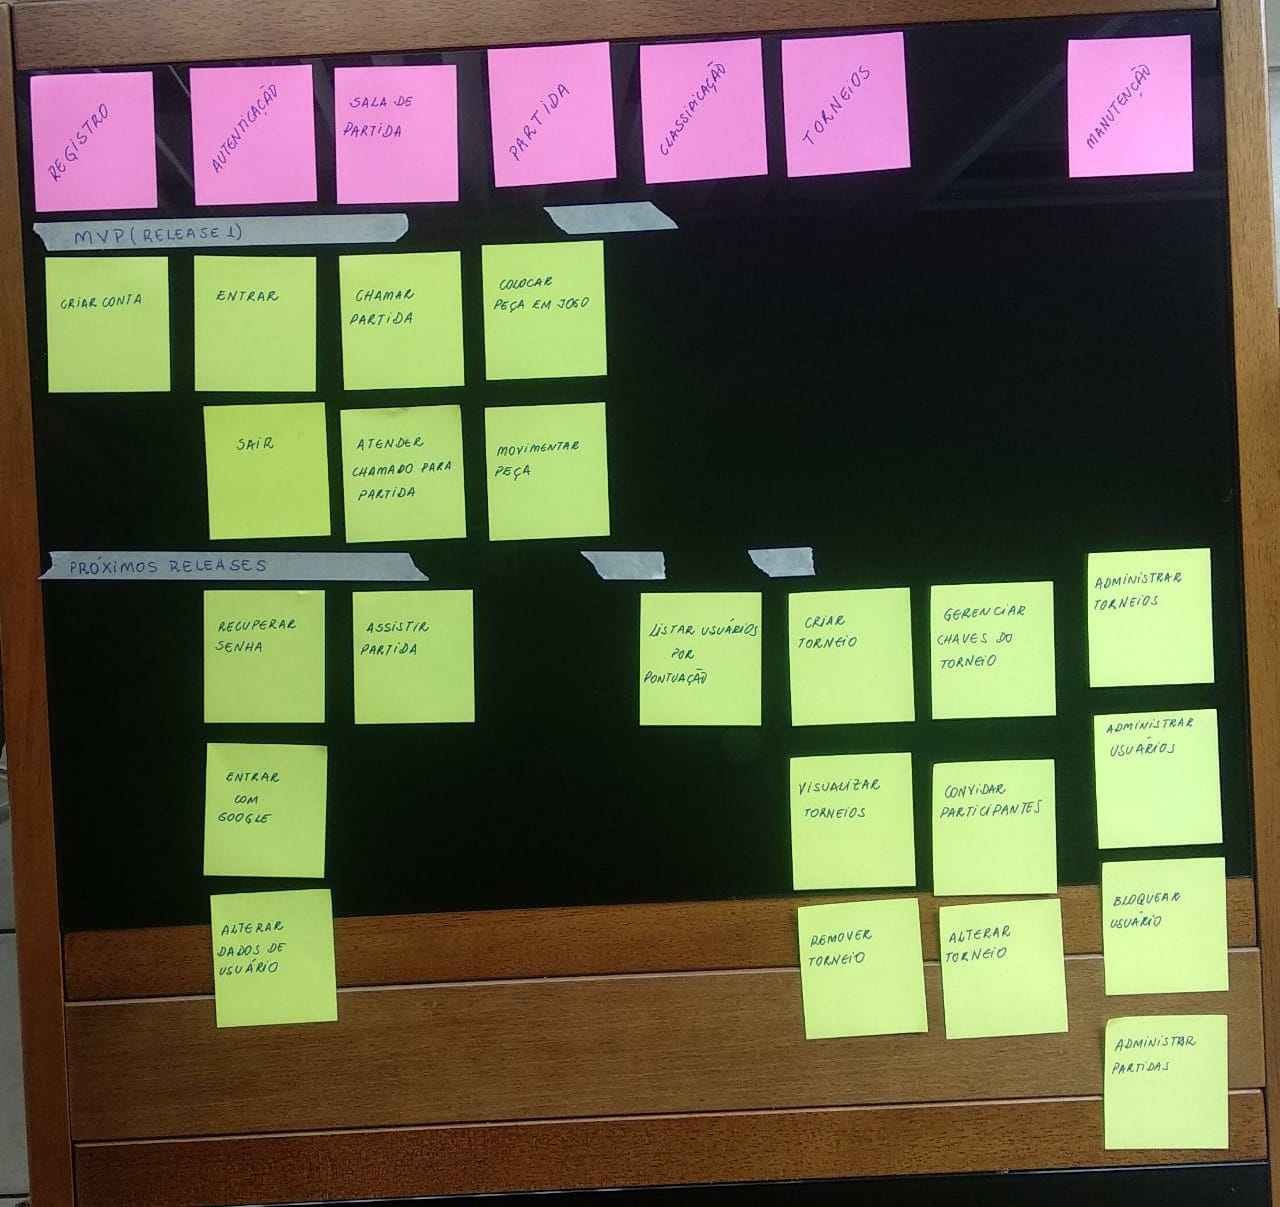
\includegraphics[width=14cm]{mapeamento-historias-usuario}
      }
    }
    Fonte: Próprio autor
    \label{fig:mapeamento-historias-usuario}
  \end{figure}

  Factualmente, existem duas escolas de TDD: \emph{Chicago} - encontrada, ainda, como inside-out (de dentro para fora), classicista, bottom-up (de baixo para cima) - e \emph{Londres} - também conhecida como outside-in (de fora para dentro), mockista, top-down (de cima para baixo). Segundo \citeonline[págs. 488-492] {BryantPerez2019}, a tecnologia utilizada, mecanismos de construção, habilidades e preferências pessoais irão determinar que abordagem escolher. Mas também cita algumas características que ajudam nesta: possui bem delineadas as regras do negócio ou terá que traduzir o processo dos interessados em regras que possam ser automatizadas; existem restrições de plataforma (deve ser uma aplicação web, deve usar um determinado servidor de banco de dados, etc).

  Sendo assim, optamos pela abordagem londrina, que tem como principais
  representantes \citeonline{FreemanPryce2009}. A primeira observação é sobre o
  ciclo que, nessa perspectiva, possui dois níveis de execução (\textbf{Figura \ref{fig:ciclo-atdd}}). Graças a isso, é esperado que a etapa mais externa permanesça por mais tempo em estado de falha.

  \begin{figure}[h]
    \centering
    \caption{Ciclo Duplo da Escola de Londres de TDD}
    \efbox{
      \makebox[\textwidth]{
        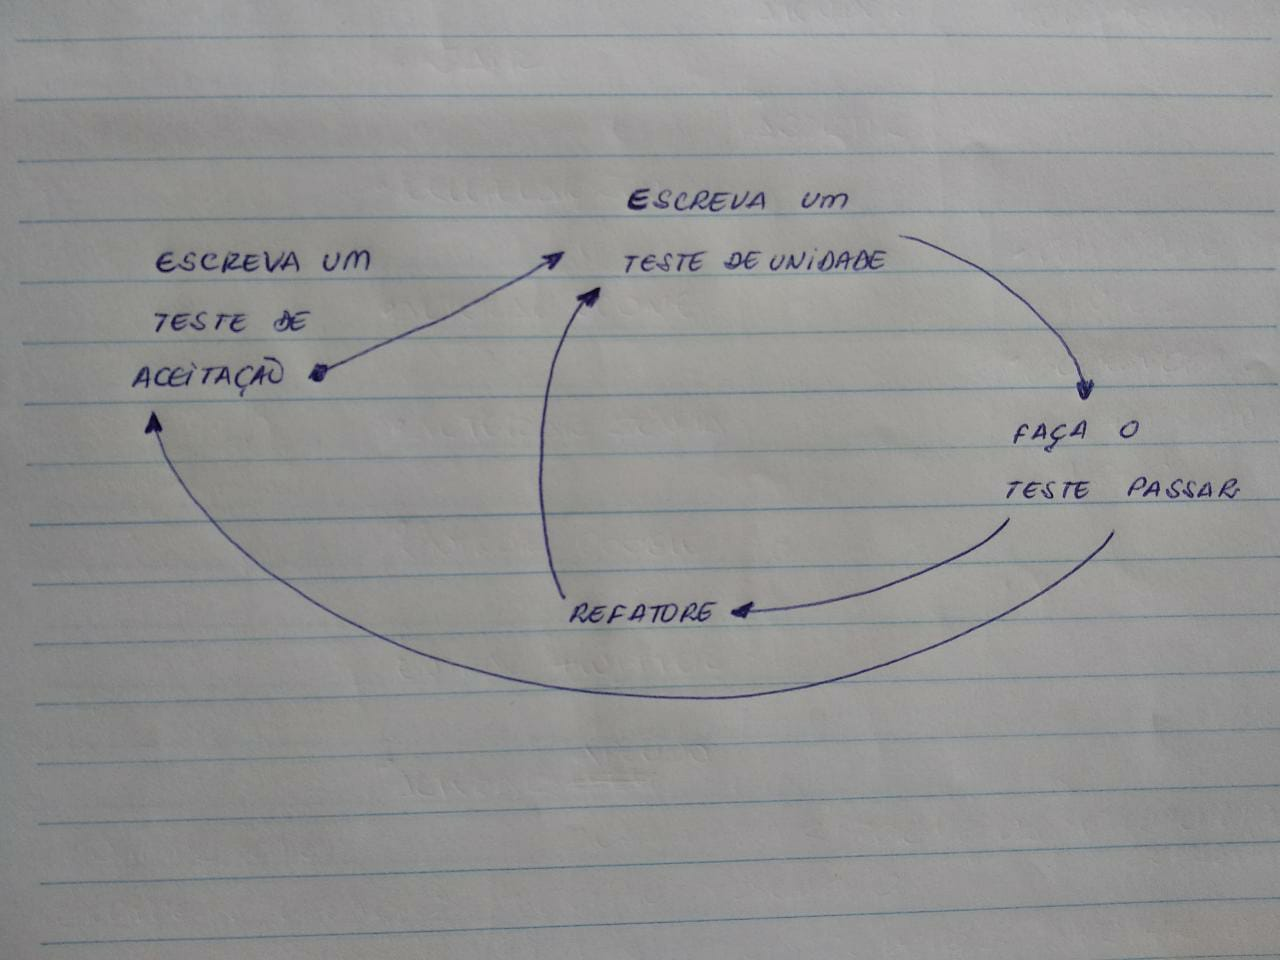
\includegraphics[width=6cm]{ciclo-atdd}
      }
    }
    Fonte: Próprio autor\footnotemark
    \label{fig:ciclo-atdd}
  \end{figure}
  \footnotetext{Baseado na imagem encontrada em \citeonline[pág. 40]
  {FreemanPryce2009}}

   Também somos forçados a definir um esboço estrutural dos componentes (\textbf{Figura \ref{fig:esboco-estrutural}}) de auto nível sobre o qual repousaremos a solução (inicialmente - pois ela pode, ou não, vir a ser modificado durante o transcorrer do projeto).

  \begin{figure}[h]
    \centering
    \caption{Esboço estrutural dos componentes da solução}
    \efbox{
      \makebox[\textwidth]{
        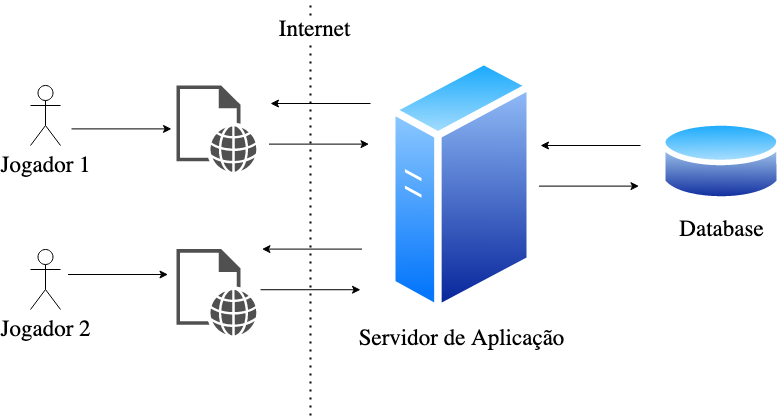
\includegraphics[width=6cm]{esboco-estrutural}
      }
    }
    Fonte: Próprio autor
    \label{fig:esboco-estrutural}
  \end{figure}
